\documentclass{ppig}
\usepackage{epsfig, graphicx} % support for image encoding and manipulation
\usepackage{ucs} % support for using UTF-8 as input encoding in LaTeX
\usepackage[utf8x]{inputenc} % required for UTF-8 support with ucs.sty
\usepackage{tabularx, multirow, booktabs} % support for high-quality tables

% The titlebox defines how much vertical space is given for
% the authors' list. If you need extra space to show all the
% authors, uncomment the line below and increase the value. Please
% do not make the titlebox smaller than the original size of 5cm.
%\setlength\titlebox{5cm}

\title{Problem-Solving in Programming: A Metacognitive Examination of IDE Design}

% List the authors like you would in a table.
% The \And command creates another author's column. Use it after the
% details of one author to separate them from the following author horizontally.
% The \AND command creates a new "row" of authors and it should be used
% when the authors don't fit on the same line. You may have to increase
% the titlebox so that the author's don't overlap with the abstract.
\author{Nicholas Nelson \\
  Electrical Engineering \&\\ Computer Science \\
  Oregon State University \\
  nelsonni@oregonstate.edu \\
  \And
  Anita Sarma \\
  Electrical Engineering \&\\ Computer Science \\
  Oregon State University \\
  Anita.Sarma@oregonstate.edu \\
  \And
  André van der Hoek \\
  Department of Informatics \\
  University of California, Irvine \\
  andre@ics.uci.edu
}
  
\date{\today}

% Packages and macros for editorial purposes. Not required for submission.
\usepackage{color}
\definecolor{darkgreen}{rgb}{0.0, 0.5, 0.0}
\definecolor{ballblue}{rgb}{0.13, 0.67, 0.8}
\definecolor{aoblue}{rgb}{0.0, 0.0, 1.0}
\newcommand{\bold}[1]{\textit{\textbf{\color{aoblue}#1}}}
\newcommand\tab[1][1cm]{\hspace*{#1}}
\usepackage{enumitem}

\begin{document}
\maketitle
\thispagestyle{empty}

\begin{abstract}

Software development encompasses more than generating, testing, and maintaining code.
It is fundamentally about harnessing cognitive problem-solving skills to develop solutions to computational problems expressed in code.
Contemporary IDEs natively support the code-centric aspects of software development, but forego providing direct support for many of the metacognitive aspects.
Examples of these metacognitive aspects include constructing models, recalling prior knowledge, interpreting code artifacts, and reflecting on work.
In this paper, we examine support in modern IDE design for three of the metacognitive problem-solving aspects: (1) articulating \& refining alternatives, (2) understanding \& assessing alternatives, and (3) recombining aspects of alternatives.
Based upon our observations, we propose a new user interface for IDEs which enables previously underrepresented aspects of problem-solving; specifically addressing the disparity in support for these three aspects. 
\end{abstract}

\bold{Section 1: scenario to illustrate programming as problem-solving\\
Section 2: introduction to column A of matrix, and details about a subset that we are focusing on in this paper\\
Section 3: challenges associated with current IDEs/problem-solving in programming\\
Section 4: envisioned solution (provide mockups and discussion about them)}

\section{Introduction}
Software developers create multiple versions of code to explore and compare viable alternative solutions.
These alternative solutions are not static artifacts that are thrown away during the next garbage cycle; they are manipulated, evaluated, broken apart, and recombined into a final version that is optimized for the requirements the developer desires most.
In many cases, the act of writing code is a small part of the larger activity that goes into solving computational problems.
Programming is not merely about language syntax and semantics~\cite{loksa2016programming}.
There are aspects of software development that involve the creation, use, and preservation of artifacts that are devoid of code.
These artifacts have a profound impact on the act of programming, the code that results from programming, and whether a developer is successful in addressing a target problem.

\bold{Scenario to illustrate programming as problem-solving\\}
To illustrate this...

Let us take the example of a team of programmers developing healthcare software which must adhere to several data security and privacy regulations.
Healthcare software used in the United States must adhere to the Health Insurance Portability and Accountability Act (HIPAA), the Healthcare Reform Act of 2010


Lets take the example.... <walk through the steps and intimate why these are problem solving steps>

Often it also involves non-coding steps. For example....

However, current IDEs focus only on one aspect/slice of programming. Restricting...causing challenges 

We take a step back to understand the different aspects of programming and current support for these.

More specifically, we focus on x and y (from Col A) since these are the steps where tool support can be the most useful

We re-think the concept of IDE to involve a card metaphor, giving the user the flexibility....We present here mockups of our prototype.
We evaluated with our folks here and found, we did awesome 

\bold{3/22/2017 input from Andre:\\
We are exploring different IDEs based on this new paradigm of programming as problem-solving.
For this exploration, we are working on a cards-based environment.
This environment is our attempt at how we think an alternative environment would function...
}



Software development encompasses more than generating, testing, and maintaining code.
It is the application of tools, techniques, and knowledge applied to problems in a software domain.
These problems could be... \bold{add two example problems that highlight both "traditional" software problems, as well as non-code based problem-solving in this same space}

\bold{
Background regarding the problem-solving traits that are well supported by modern IDEs:
	\begin{itemize}[noitemsep, nolistsep]
	\item	Translating strategies to actions
	\item	Tracking progress
	\item	Evaluating and assessing change
	\item	Synchronization
	\item	...and others from PPS-Matrix
	\end{itemize}}
	
Not all aspects of problem-solving are as explicit as these, and in fact particular, it is the implicit elements of problem-solving that have less support from modern IDEs.

\bold{
Background regarding the problem-solving traits that are not well supported by modern IDEs:
	\begin{itemize}[noitemsep, nolistsep]
	\item	Articulating/refining alternatives
	\item	Recombining aspects of alternatives
	\item	Constructing models
	\item	Leveraging group knowledge
	\item	...and others from PPS-Matrix
	\end{itemize}}
	
Traditional IDEs are built for particular programming languages, use cases, and workflows.
Adding support for new languages and use cases to these IDEs increases UI complexity, but it does not cause a shift in the underlying design.
And for the sake of performance and consistency, uniformity is maintained across different UI components by tightly coupling the UI model with the IDE's internal infrastructure.
This coupling results in rigidity in the workflows allowed within a particular IDE.
Experimentation in alternative UI, workflow models, and use cases have higher intrinsic costs because of this IDE design mentality.

\section{Problem-Solving in Programming}
In the context of programming, the language of problem-solving must transition from the generic nature described in psychology literature~\bold{mayer1992thinking} to a domain-specific language that exemplifies the particular activities involved.
We present a model of the activities, and underlying actions, that occur when developers use code as a medium to resolve computation problems.
Table~\ref{matrix} contains our model, characterized into \textit{Activities} that are generic to problem-solving but have an analogous element within programming, and the \textit{Actions} that constitute direct programming actions taken in pursuit of solutions to programming tasks.

\begin{table}[!htbp]
\caption{Problem-Solving in Programming: Activities and Actions}
\label{matrix}
\centering
\begin{tabular}{|c|l|}
	\hline
	\multicolumn{1}{|c|}{\textbf{Activity}} 
	& \multicolumn{1}{c|}{\textbf{Action}}\\\hline
	\multirow{5}{*}{Understanding the situation} 
	& Identifying goals \\\cline{2-2}
	& Recalling prior knowledge \\\cline{2-2}
	& Constructing models \\\cline{2-2}
	& Interpreting code artifacts \\\cline{2-2}
	& Filling knowledge gaps \\\hline
	Externalizing thoughts \& ideas 
	& Representing relevant information \\\hline
	\multirow{4}{*}{Developing strategies} 
	& Generating alternatives \\\cline{2-2}
	& Articulating and refining alternatives \\\cline{2-2}
	& Understanding and assessing alternatives \\\cline{2-2}
	& Recombining aspects of alternatives \\\hline
	\multirow{3}{*}{Enacting change} 
	& Translating strategies to actions \\\cline{2-2}
	& Tracking progress \\\cline{2-2}
	& Evaluating and assessing change \\\hline
	\multirow{5}{*}{Collaborate} 
	& Feedback solicitation \\\cline{2-2}
	& Team work \\\cline{2-2}
	& Group think \\\cline{2-2}
	& Leveraging group knowledge \\\cline{2-2}
	& Synchronization \\\hline
	\multirow{2}{*}{Retrospect} 
	& Reflect on work \\\cline{2-2}
	& Preserve work \\\hline
\end{tabular}
\end{table}

For example, when a developer has gathered enough information to be informed about a particular problem, they will begin to developer strategies for resolving that problem.
Developers will \textit{generate alternatives}, \textit{articulate and refine those alternatives} in order to verify that they appropriately communicate the distinct elements of each alternative, seek to \textit{understand and assess the alternatives} to determine rationales for and against each, and finally \textit{separate and recombine aspects of alternative} strategies that optimizes for desired properties of execution and the final product.

We conjecture that each of the actions in Table~\ref{matrix} represent aspects of programming when examined through the lens of problem-solving.
Each action is not required individually, but a minimum subset allows for successful programming sessions that produce code that solves the computational problem targeted.

\section{Challenges}
\bold{Weave references to Code Bubbles/Debugger Canvas and PatchWorks as part of the challenges discussions, since it is particularly relevant to our concepts.}

\bold{3/15/2017 input from Anita:
	\begin{itemize}[noitemsep, nolistsep]
	\item	C1: code centric
	\item	C2: not geared towards dynamic exploration / backtracking / breadcrumbs
	\subitem C1.1: past history
	\subitem C1.2: immediate past exploration
	\subitem C1.3: Outside resources
	\item	C3: evaluate options (side-by-side)
	\item	C4: flexible to match individual's programming preferences
	\item	C5: currently only code is considered 1st class; consider all pieces equivalent
	\subitem based on context of current work, diff aspects of project might take precedence
	\end{itemize}
}

\bold{
Modern IDEs don't support all problem-solving aspects.
	\begin{itemize}[noitemsep, nolistsep]
	\item	IDEs are highly-coupled to a code-centric metaphor of software development.
	\item	IDEs are built around workflows that fit for only certain languages (ex: Java-specific for Eclipse/IntelliJ).
	\item	IDEs are NOT general-purpose programming environments (ex: RStudio, PyCharm, etc.).
	\item	The UI layer is dictated by both the target programming language and the typical use-case (see point above).
	\item	Experimentation in UI design, and by association certain workflows, are not supported by most IDEs.
	\item	Problem-solving tasks unrelated to code are typically banished to plugins or not supported at all.
	\end{itemize}}

\section{Bonsai IDE}
To address these challenges, we present Bonsai IDE, an integrated development environment for problem-solving in software development.
The goal of Bonsai IDE is to offer developers: a cards-based interface for organizing and searching artifacts based on changing requirements, and an extensible catalog of card UI elements that can easily accommodate new use-cases and behaviors.
This approach provides developers with a framework for adapting their IDE to suit their desired configuration, instead of adapting their processes to compensate for it.

\subsection{Cards}
\fbox{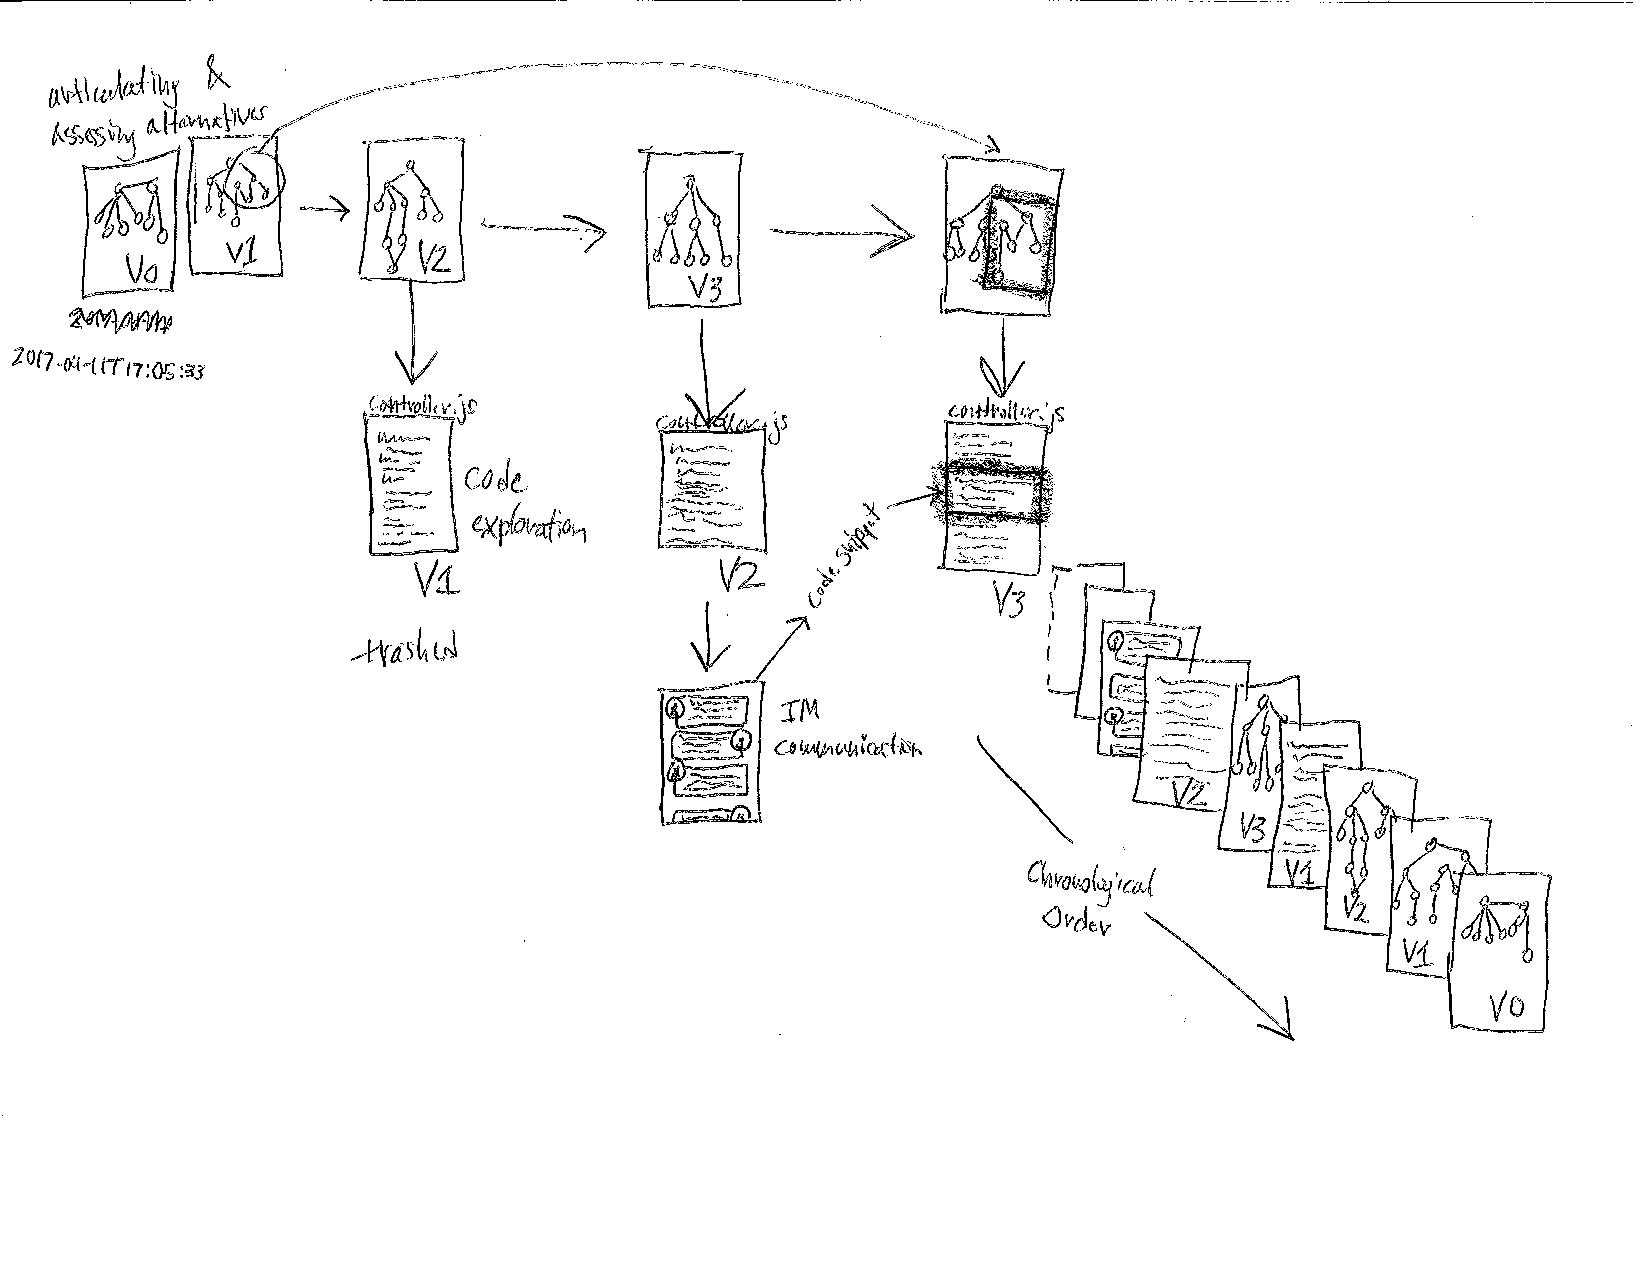
\includegraphics[trim={0 3.5cm 1.0cm 0.6cm},clip,width=\textwidth]{Mockup-7}}
\bold{Discussion of elements in the code card figure above.}

\bold{FIGURE: Front and back of a non-code card (web-search results?).}
\bold{Discussion of elements in the non-code card figure above.}

\bold{
Cards have the following properties:
	\begin{itemize}[noitemsep, nolistsep]
	\item 	Moveable anywhere across the IDE canvas window.
	\item 	Individual cards are not resizable, however user settings should allow for increasing the default size of all cards.
	\item 	Each card allows for the expansion to a full-screen mode to accommodate editing the entire content of a cards (since cards are likely to be too small of an editable workspace).
	\item 	Discussion about the meta-data contained on the reverse of a card.
	\item 	Use examples of a code-based card (OO languages lend themselves to cards in the easiest to understand manner), and also non-code cards such as developer notes from a meeting (i.e. informal requirements) and web-search results from StackOverflow (answers with code references for better applicability).
	\end{itemize}
}

\subsection{Canvas}
\bold{FIGURE: Basic canvas with a few cards in both stacked and fully-exposed sets, as well as a few unorganized cards.}
\bold{Discussion of the different organizational elements in the figure above.}

\bold{
Canvas has the following properties:
	\begin{itemize}[noitemsep,nolistsep]
		\item	Size is infinite in all directions.
		\item	Cards cannot be farther than 1-screen distance from any other cards; prevents losing cards in the ether of infinite area.
		\item	Cards can be stacked in piles throughout the canvas.
		\item	Filtering allows new groupings (stacks, hand of cards, or fully-exposed set) based upon user-defined criteria.
		\item	Filtering criteria could include: most recent, only cards edited by Joe, only cards not currently pushed to a non-local version control system, all cards that contained errors according to the last compilation/build/execution attempt, etc.
		\item	Search allows cards to remain where they have been placed, but assists the user in navigating to that particular location (via card highlighting, or some similar UI element).
	\end{itemize}
}

\section{Conclusions}
Our conclusions are ...


\section{Acknowledgements}
\bold{Add any NSF, OSU, UCI, etc. grants or funding references as needed.}

\bibliography{bibliography}
\bibliographystyle{apacite} 
\end{document}
